%!TEX output_directory = texaux
%!TEX spellcheck
%!TEX root = ../main.tex

\setlength{\abovedisplayskip}{20pt}
\setlength{\belowdisplayskip}{20pt}

\chapter{Odpowiadanie na pytania} \label{rozdzial4}

Poprzednio opisane mechanizmy budowały model ogólnej rozmowy. Bot był bardzo ograniczony w swojej umiejętności rozumienia tekstu. Jego odpowiedzi co prawda zwykle pasowały do kontekstu, ale niewiele więcej można o nich powiedzieć. Większość systemów dialogowych powstaje z myślą o konkretnym celu, do którego zrealizowania nie wystarczy prowadzenie ``rozmowy o niczym''. Użyteczny robot może na przykład być w~stanie dostarczyć człowiekowi wartościowych informacji. W tym rozdziale przedstawiam kolejne wyzwanie chatbotów, które może być rozwiązane za pomocą sieci neuronowej.

Chcemy nauczyć program odpowiadania na pytania o fakty formułowane w~języku naturalnym. Przykładem może być \textit{When was Battle of Grunwald?}. Sama analiza występowania słów tutaj nie wystarczy, musimy zaopatrzyć model w jakieś źródło wiedzy. Tym źródłem będzie krótki tekst w języku naturalnym. Naszym celem jest sprawić, by bot na powyższe pytanie odpowiedział poprawnie po przeczytaniu tekstu, który może wyglądać tak:\\

\small\textit{The Battle of Grunwald, First Battle of Tannenberg or Battle of Žalgiris, was fought on 15 July 1410 during the Polish–Lithuanian–Teutonic War. The alliance of the Kingdom of Poland and the Grand Duchy of Lithuania, led respectively by King Władysław II Jagiełło (Jogaila) and Grand Duke Vytautas, decisively defeated the German–Prussian Teutonic Knights, led by Grand Master Ulrich von Jungingen.}\footnote{Fragment pochodzi z \url{https://en.wikipedia.org/wiki/Battle_of_Grunwald}}\\

\normalsize
Powyższy problem cieszy się rosnącym zainteresowaniem wśród społeczności zajmujących się uczeniem maszynowym. W 2016 roku opublikowany został \textit{Stanford Question Answering Dataset (SQuAD)} \cite{squaddata}, zbiór danych zawierający blisko 86\,000 pytań. Do każdego pytania dołączony jest krótki fragment stanowiący kontekst. Skuteczność na \textit{SQuAD}zie jest popularną miarą jakości systemów odpowiadających na pytania o fakty. W ostatnim czasie najlepsze z nich niemalże dorównały umiejętnościom człowieka\footnote{\url{https://rajpurkar.github.io/SQuAD-explorer/}}.

W momencie przygotowywania tej pracy jedno z czołowych miejsc w rankingu \textit{SQuAD} zajmował system \textit{FastQA} \cite{fastqa}. Dalsza część rozdziału zawiera opis, przykłady zastosowania, i przedstawienie próby usprawnienia tego systemu.

%%%%%%%%%%%%%%%%%%%%%%%%%%%%%%%%%%%%%%%%%%%%%%%%%%%%%%%%%%%%%%%%%%%%%%%%%

\section{FastQA}

Jak wiele innych modeli tego typu, \textit{FastQA} odpowiada cytując pewien podciąg kontekstu. Dla każdego pytania $q = q_1^{K_q}$ w zbiorze uczącym mamy odpowiadający mu tekst $x = x_1^{K_x}$ oraz parę indeksów $\mathbf{s}, \mathbf{e} \in \{1,\dots,K_x\}$ takich, że $x_{\mathbf{s}}^{\mathbf{e}}$ jest poprawną odpowiedzią. Ucząc model staramy się maksymalizować prawdopodobieństwo wybrania właściwego ciągu, czyli
\[\hat{P}_s(\mathbf{s} \mid q, x)\ \hat{P}_e(\mathbf{e} \mid \mathbf{s}, q, x).\]

%%%%%%%%%%%%%%%%%%%

\subsection{Architektura sieci}

Podstawowy pomysł polega na zakodowaniu pytania i kontekstu za pomocą sieci rekurencyjnej, a następnie wykorzystaniu uzyskanej informacji do obliczenia $P_s$,~$P_e$~--~rozkładów prawdopodobieństwa na $\{1,\dots,K_x\}$. Można zrealizować go tak:

\begin{enumerate}
    \item \textbf{Zanurzenia}: zanurzamy $q$ jako $v_1^{K_q}$ i $x$ jako $u_1^{K_x}$.
    \item \textbf{Kodujący \textit{RNN}}: zamieniamy $v_1^{K_q}$ na ciąg wektorów $z_1^{K_q}$ oraz $u_1^{K_x}$ na $h_1^{K_x}$.
    \item \textbf{Reprezentacja pytania}: w pewien sposób agregujemy ciąg $z_1^{K_q}$ do jednego wektora $\tilde{z}$ reprezentującego pytanie.
    \item \textbf{Początki}: do każdego $h_i$ dodajemy informację o $\tilde{z}$, aby powiązać pytanie z~kontekstem. Powstaje ciąg ${h'}_1^{K_x}$. Wektory $h'_i$ są zwijane do skalarów. Funkcja \textit{softmax} nałożona na wynik daje prawdopodobieństwa $\hat{P}_s(i \mid q, x)$ dla $i \in \{1,\dots,K_x\}$.
    \item \textbf{Końce}: każde $h'_i$ wzbogacamy dodatkowo o $h_{\mathbf{s}}$ tworząc ciąg ${h''}_1^{K_x}$. Ciąg ten zwijamy do ciągu skalarów, po czym nakładamy \textit{softmax}. W ten sposób otrzymujemy wartości $\hat{P}_e(i \mid \mathbf{s}, q, x)$.
\end{enumerate}

\begin{figure}[H]
  \centering
    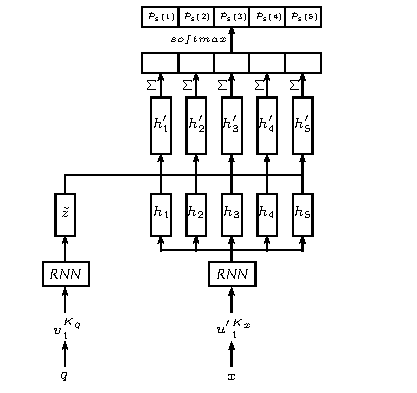
\includegraphics[width=0.9\textwidth]{chapter4/img/fastqa.eps}
  \caption{\small{Uproszczony schemat \textit{FastQA}. Dla czytelności przedstawione jest tylko obliczanie $\hat{P}_s$}. Wektory $u'_i$ to ostateczne reprezentacje słów kontekstu, po dołączeniu zanurzeń znakowych i dwóch dodatkowych cech opisanych poniżej.}
  \label{rysfqa}
\end{figure}

%%%%%%%%%%%%%%%%%%%

\subsubsection{Dodatkowe cechy słów}

Najważniejszą nowością wprowadzaną przez \textit{FastQA} są dwie dodatkowe cechy dla słów kontekstu. Dla każdego $x_i$ są one obliczane na podstawie zależności między $x_i$ a $q$. Okazuje się, że prosta heurystyka mówiąca jak istotne jest dane słowo dla pytania bardzo pomaga podnieść jakość modelu.

Autorzy proponują cechy binarną i ważoną. Binarna stanowi informację o tym, czy słowo znajduje się w pytaniu. Dla $i \in \{1,\dots,K_x\}$:

\[f_b(i, q) =
    \begin{cases}
        1 & \text{jeśli } x_i \text{ występuje w } q \\
        0 & \text{w p.p.} \\[5pt]
    \end{cases}
\]

Przy obliczaniu cechy ważonej najpierw tworzymy macierz podobieństwa pomiędzy słowami kontekstu a słowami pytania. Podobieństwa te są normalizowane funkcją \textit{softmax} i~sumowane po całym $q$.

\[
\begin{aligned}
    \mathrm{sim}_{i,j} &= {\tau_w}^T (u_i \odot v_j) \in \mathbb{R} \\[3pt]
    f_w(i, q) &= \sum\limits_{j \in \{1,\dots,K_q\}} (\mathrm{softmax}(\mathrm{sim}_{\,\cdot,\,j}))_i \\[5pt]
\end{aligned}
\]

\noindent
gdzie $\tau_w \in \mathbb{R}^n$ dla wymiaru zanurzeń $n$. Symbol $^T$ oznacza transpozycję. Parametr $\tau_w$ jest uczony wraz z resztą sieci. Dla każdego $i \in \{1,\dots,K_x\}$ wartości $f_b(i, q)$ i~$f_w(i,q)$ są doklejane do reprezentacji słowa $x_i$ w kroku~1 tworząc zaznaczony na Rysunku~\ref{rysfqa} ciąg ${u'}_1^{K_x}$.

%%%%%%%%%%%%%%%%%%%

\subsubsection{Reprezentacja pytania}

Istotnym elementem modelu jest sposób wyliczania podsumowania pytania, $\tilde{z}$. Wykorzystywany jest do tego tzw. \textit{mechanizm uwagi} (ang. \textit{attention}). Poszczególne wektory ciągu $z_1^{K_q}$ są sumowane z wagami oznaczającymi ich istotność w pytaniu. Odbywa się to podobnie jak w przypadku obliczania $f_w$. Niech $Z = [z_1\ \cdots\ z_{K_q}] \in \mathbb{R}^{m \times K_q}$, gdzie $m$ jest rozmiarem stanu \textit{RNN}:

\[
\begin{aligned}
    \alpha &= \mathrm{softmax}({\tau_q}^T Z) \in \mathbb{R}^{K_q} \\[3pt]
    \tilde{z} &= \sum\limits_{j \in \{1,\dots,K_q\}} \alpha_j z_j \\[5pt]
\end{aligned}
\]

Parametr $\tau_q \in \mathbb{R}^m$ jest uczony. Wykorzystując taką reprezentację $q$ sieć potrafi nauczyć się zwracać uwagę na specyficzne słowa. Na przykład obserwując wiele pytań rozpoczynających się od \textit{when} i mających daty za odpowiedzi, będzie w stanie tak dobrać parametry, żeby słowo \textit{when} dostawało dużą wagę. W praktyce typ pytania mocno ogranicza zakres możliwych odpowiedzi. Mechanizm uwagi pozwala modelowi wykorzystywać ten fakt.

%%%%%%%%%%%%%%%%%%%

\subsubsection{Zanurzenia znakowe}

Zanurzać w przestrzeni wektorowej można nie tylko słowa, ale także pojedyncze znaki. \textit{FastQA} korzysta zarówno z zanurzeń słów jak i z reprezentacji liter. Niech $w$ będzie słowem złożonym ze znaków $c_1,\dots,c_l$, a $m_c$ rozmiarem zanurzeń liter. Możemy zapisać $w$ jako $A = [a_1\ \cdots\ a_l] \in \mathbb{R}^{m_c \times l}$, gdzie $a_i$ jest wektorem dla $c_i$. Macierz $A$ przekształcamy na wektor stałej długości, który będzie reprezentacją $w$ uwzględniającą wzajemne położenie liter w słowie \cite{charemb}.

Wykorzystujemy do tego operację splotu. Dla filtra $H \in \mathbb{R}^{m_c \times k}, k \leq l$ i~opcjonalnego przesunięcia $b \in \mathbb{R}$ definiujemy $A*H \in \mathbb{R}^{l-k+1}$ następująco:
\[(A*H)_i = \tanh(\mathrm{tr}([a_i\ \cdots\ a_{i+k-1}]H^T) + b)\]

Interesującym nas rezultatem jest skalar $\max(A*H)$. Całą operację powtarzamy dla pewnej liczby $n_f$ różnych filtrów, a otrzymane wyniki łączymy w $n_f$-wymiarowy wektor reprezentujący $w$. Wektor ten jest doklejany do zanurzenia $w$ w kroku 1, przed dodaniem cech $f_b$ i $f_w$.

Aby zapewnić dodatkową interakcję pomiędzy dwoma typami zanurzeń słów, autorzy wykorzystują warstwę \textit{highway} \cite{highway}. Niech $\mathbf{w} \in \mathbb{R}^{n+n_f}$ będzie konkatenacją obu reprezentacji $w$. Podlega ona następującym transformacjom:

\[
\begin{aligned}
\mathbf{w}' &= P\mathbf{w}\\
g &= \mathcal{F}_1(\mathbf{w}')\\
\mathbf{w}'' &= \mathcal{F}_2(\mathbf{w}')\\
\tilde{\mathbf{w}} &= g \odot \mathbf{w}' + (1-g) \odot \mathbf{w}'',
\end{aligned}
\]

\noindent
gdzie $P$ jest pewną macierzą, $\mathcal{F}_1$ i $\mathcal{F}_2$ oznaczają warstwy gęste, a $\tilde{\mathbf{w}}$ jest powstałą reprezentacją $w$, do której konkatenowane będą $f_b$ i $f_w$. Warstwa \textit{highway} potrafi nauczyć się proporcji w jakich powinna brać pod uwagę oryginalne i przekształcone wejście.

%%%%%%%%%%%%%%%%%%%

\subsubsection{Pozostałe szczegóły}

W krokach 4. i 5. do kodowania kontekstu dołączamy dodatkowe informacje, które chcemy uwzględnić przy obliczaniu prawdopodobieństw. Najprościej zrobić to przez konkatenację, ale autorzy dołączają dodatkowo iloczyn Hadamarda:

\[
\begin{aligned}[c]
    h'_i &=
    \begin{bmatrix}
        h_i \\
        \tilde{z} \\
        h_i \odot \tilde{z} \\
    \end{bmatrix} \in \mathbb{R}^{3m}
\end{aligned} \ \
\begin{aligned}[c]
    h''_i &=
    \begin{bmatrix}
        h_i \\
        h_{\mathbf{s}} \\
        \tilde{z} \\
        h_i \odot \tilde{z} \\
        h_i \odot h_{\mathbf{s}} \\
    \end{bmatrix} \in \mathbb{R}^{5m}
\end{aligned}
\]


Wektory $h'_i$ oraz $h''_i$ są zwijane do skalarów za pomocą podwójnej warstwy gęstej. Funkcja \textit{softmax} zwraca prawdopodobieństwa:

\[
\begin{aligned}
    &s_i = {\tau_s}^T \mathrm{ReLU}(W_s h'_i + b_s) \in \mathbb{R}\\
    &\hat{P}_s(i \mid q, x) = (\mathrm{softmax}(s))_i \\[10pt]
    &e_i = {\tau_e}^T \mathrm{ReLU}(W_e h''_i + b_e) \in \mathbb{R}\\
    &\hat{P}_e(i \mid \mathbf{s}, q, x) = (\mathrm{softmax}(e))_i\\[5pt]
\end{aligned}
\]

Jako warstwę rekurencyjną, kodującą pytanie i kontekst, wykorzystano dwukierunkowy \textit{LSTM} (\ref{lstm}, \ref{birnn}). Agregację wyników sieci składowych przeprowadzono za pomocą przepuszczenia połączonych stanów przez warstwę gęstą o parametrze $B \in \mathbb{R}^{m \times 2m}$ (bez przesunięcia). Przetwarzanie $q$ i $x$ zostało przeprowadzone za pomocą tych samych parametrów, za wyjątkiem macierzy $B$, która była inna dla pytania i kontekstu. Wartości cech $f_b$~i~$f_w$ dla słów w pytaniu zostały ustalone na 1.

Warstwa zanurzeń podlega procedurze \textit{dropout} \cite{dropout}. Jest to popularna i prosta metodą regularyzacji modelu neuronowego. Każdy element wejścia podlega wyzerowaniu z prawdopodobieństwem $p$, a następnie całość jest mnożona przez $1\, /\, (1-p)$, żeby zachować stałą średnią wyniku. W ten sposób symulujemy uśrednianie wielu modeli. Częstym wyborem $p$ jest $0.5$.

%%%%%%%%%%%%%%%%%%%%%%%%%%%%%%%%%%%%%%%%%%%%%%%%%%%%%%%%%%%%%%%%%%%%%%%%%

\section{Eksperymenty}

Model został wyuczony procedurą \textit{ADAM} (\ref{adam}) na danych \textit{SQuAD}. Wykorzystane zanurzenia słów pochodzą z GloVe i nie były uczone. Zanurzenia znakowe zostały wytrenowane. Co 64\,000 elementów znajdował się punkt kontrolny. Jeśli efektywność na zbiorze testowym malała między punktami kontrolnymi, tempo uczenia było zmniejszane dwukrotnie. Cały proces był dość szybki: 20 przejść po całym zbiorze uczącym zajęło około 4 godziny. Najlepszy rezultat pojawił się już po 9 przejściach.

Miarą jakości modelu jest procent poprawnie udzielonych odpowiedzi na zbiorze testowym. Oficjalny skrypt ewaluacyjny oblicza również miarę F1, stanowiącą balans pomiędzy precyzją (ang. \textit{precision}) i czułością (ang. \textit{recall}). Niestety nie udało mi się zreplikować wyniku z \cite{fastqa}. Model uzyskał 72.34 F1, co jest wynikiem trochę niższym od 76.30 F1 prezentowanym w artykule. Powodem mogą być pojawiające się tam drobne niejasności, które mogłem źle zinterpretować. Nie wykluczam oczywiście błędnej implementacji, chociaż nie potrafiłem znaleźć żadnej usterki. Nie mniej jednak otrzymany wynik jest wystarczająco dobry, żeby przekonać się jak sieć sprawdza się w praktyce.

%%%%%%%%%%%%%%%%%%%

\subsection{Przykłady zastosowania}

Wytrenowana sieć stara się znaleźć podciąg kontekstu, który z największym prawdopodobieństwem jest dobrą odpowiedzią. Sprawdzenie wszystkich możliwych podciągów jest niepraktyczne, więc stosuje się przeszukiwanie wiązkowe (\ref{beamsearch}). Zmniejszenie rozmiaru wiązki do 1 skutkuje jednak dużo szybszym algorytmem zachłannym, który działa tylko nieznacznie gorzej. Takiej właśnie wersji używam.

W tej części zamieszczam przykładowe odpowiedzi udzielone przez model. W~nawiasach znajdują się zwrócone prawdopodobieństwa. Wartości bliskie 1 oznaczają, że sieć jest pewna odpowiedzi. Mniejsze liczby sygnalizują trudniejsze przypadki. Pytania i konteksty pochodzą ze zbioru testowego \textit{SQuAD}. Błędne odpowiedzi są opatrzone dodatkowymi komentarzami.\\\\

%!TEX output_directory = texaux
%!TEX spellcheck
%!TEX root = ../main.tex

\setlength{\abovedisplayskip}{20pt}
\setlength{\belowdisplayskip}{20pt}

\small
\noindent
\textbf{Kontekst}:
\textit{Other green spaces in the city include the Botanic Garden and the University Library Garden. They have extensive botanical collection of rare domestic and foreign plants, while a palm house in the New Orangery displays plants of subtropics from all over the world. Besides, within the city borders, there are also: Pole Mokotowskie (a big park in the northern Mokotów, where was the first horse racetrack and then the airport), Park Ujazdowski (close to the Sejm and John Lennon street), Park of Culture and Rest in Powsin, by the southern city border, Park Skaryszewski by the right Vistula bank, in Praga. The oldest park in Praga, the Praga Park, was established in 1865–1871 and designed by Jan Dobrowolski. In 1927 a Zoological Garden (Ogród Zoologiczny) was established on the park grounds, and in 1952 a bear run, still open today.}

\noindent
\textbf{P}: \textit{What type of space in Warsaw are the Botanic Garden and University Library Garden?}\\
\textbf{O}: \textit{green} (0.81)\\[4pt]
\textbf{P}: \textit{Where is a palm house with subtropic plants from all over the world on display?}\\
\textbf{O}: \textit{New Orangery} (0.35)\\[4pt]
\textbf{P}: \textit{Where was the first horse racetrack located?}\\
\textbf{O}: \textit{pole mokotowskie} (0.34)\\[4pt]
\textbf{P}: \textit{What park is close to John Lennon street?}\\
\textbf{O}: \textit{park ujazdowski} (0.95)\\[4pt]
\textbf{P}: \textit{When was a zoological garden established in the Praga Park?}\\
\textbf{O}: \textit{1865 – 1871} (0.77) (błąd, poprawna odpowiedź: \textit{1927})

\vspace{.3cm}

\noindent
\textbf{Kontekst}:
\textit{Following the cretaceous–paleogene extinction event , the extinction of the dinosaurs and the wetter climate may have allowed the tropical rainforest to spread out across the continent. From 66–34 mya, the rainforest extended as far south as 45\degree. Climate fluctuations during the last 34 million years have allowed savanna regions to expand into the tropics. During the oligocene, for example, the rainforest spanned a relatively narrow band. It expanded again during the middle miocene, then retracted to a mostly inland formation at the last glacial maximum. However, the rainforest still managed to thrive during these glacial periods, allowing for the survival and evolution of a broad diversity of species.}

\noindent
\textbf{P}: \textit{Which type of climate may have allowed the rainforest to spread across the continent?}\\
\textbf{O}: \textit{tropical} (0.52) (błąd, poprawna odpowiedź: \textit{wetter})\\[4pt]
\textbf{P}: \textit{What has allowed for the savanna region to expand into the tropics?}\\
\textbf{O}: \textit{climate fluctuations} (0.98)\\[4pt]
\textbf{P}: \textit{During what time did the rainforest spanned a narrow band?}\\
\textbf{O}: \textit{the oligocene ,} (0.20) (nieścisłość: niepotrzebny przecinek)\\[4pt]
\textbf{P}: \textit{When did it retract to a inland formation?}\\
\textbf{O}: \textit{middle miocene} (0.49)\\[4pt]
\textbf{P}: \textit{Did the rainforest managed to thrive during the glacial periods?}\\
\textbf{O}: \textit{still managed to thrive} (0.31)

\vspace{.3cm}

\noindent
\textbf{Kontekst}:
\textit{QuickBooks sponsored a ``Small Business Big Game'' contest, in which Death Wish Coffee had a 30-second commercial aired free of charge courtesy of QuickBooks. Death Wish Coffee beat out nine other contenders from across the United States for the free advertisement.}

\noindent
\textbf{P}: \textit{What company won a free advertisement due to the QuickBooks contest?}\\
\textbf{O}: \textit{coffee} (0.34) (niepełna odpowiedź, poprawna: \textit{death wish coffee})\\[4pt]
\textbf{P}: \textit{How long was the Death Wish Coffee commercial?}\\
\textbf{O}: \textit{30 - second} (0.78)\\[4pt]
\textbf{P}: \textit{Besides Death Wish Coffee, how many other competitors participated in the contest?}\\
\textbf{O}: \textit{nine} (0.63)\\[4pt]
\textbf{P}: \textit{Which company sponsored a contest called ``Small Business Big Game''?}\\
\textbf{O}: \textit{quickbooks} (1.0)\\[4pt]
\textbf{P}: \textit{How many other contestants did the company, that had their ad shown for free, beat out?}\\
\textbf{O}: \textit{nine} (0.80)

% \vspace{.3cm}

% \noindent
% \textbf{Kontekst}:
% \textit{Despite waiving longtime running back Deangelo Williams and losing top wide receiver Kelvin Benjamin to a torn ACL in the preseason, the Carolina Panthers had their best regular season in franchise history, becoming the seventh team to win at least 15 regular season games since the league expanded to a 16-game schedule in 1978. Carolina started the season 14–0, not only setting franchise records for the best start and the longest single-season winning streak, but also posting the best start to a season by an NFC team in NFL history, breaking the 13–0 record previously shared with the 2009 New Orleans Saints and the 2011 Green Bay Packers. With their NFC-best 15–1 regular season record, the Panthers clinched home-field advantage throughout the NFC playoffs for the first time in franchise history. Ten players were selected to the Pro Bowl (the most in franchise history) along with eight all-pro selections.}

% \noindent
% \textbf{P}: \textit{Who had the best record in the NFC?}\\
% \textbf{O}: \textit{carolina panthers} (0.39)\\[4pt]
% \textbf{P}: \textit{How many Panthers went to the Pro Bowl?}\\
% \textbf{O}: \textit{ten} (0.74)\\[4pt]
% \textbf{P}: \textit{What Panther tore his ACL in the preseason?}\\
% \textbf{O}: \textit{kelvin benjamin} (0.94)\\[4pt]
% \textbf{P}: \textit{What year did the league begin having schedules with 16 games in them?}\\
% \textbf{O}: \textit{1978} (0.99)\\[4pt]
% \textbf{P}: \textit{What year did the the Saints hit a 13-0 record?}\\
% \textbf{O}: \textit{2009} (0.94)

\vspace{.3cm}

\noindent
\textbf{Kontekst}:
\textit{Sir Charles Lyell first published his famous book, Principles of Geology, in 1830. This book, which influenced the thought of Charles Darwin, successfully promoted the doctrine of uniformitarianism. This theory states that slow geological processes have occurred throughout the Earth's history and are still occurring today. In contrast, catastrophism is the theory that Earth's features formed in single, catastrophic events and remained unchanged thereafter. Though Hutton believed in uniformitarianism, the idea was not widely accepted at the time.}

\noindent
\textbf{P}: \textit{First published by Sir Charles Lyell in 1830 this book was called what?}\\
\textbf{O}: \textit{principles of geology} (0.96)\\[4pt]
\textbf{P}: \textit{What doctrine did the doctrine of the Principles of Geology successfully promote?}\\
\textbf{O}: \textit{the doctrine of uniformitarianism} (0.63)\\[4pt]
\textbf{P}: \textit{Which theory states that slow geological processes are still occurring today, and have occurred throughout Earth's history?}\\
\textbf{O}: \textit{uniformitarianism} (0.48)\\[4pt]
\textbf{P}: \textit{Which theory states that Earth's features remained unchanged after forming in one single catastrophic event?}\\
\textbf{O}: \textit{catastrophis}m (1.0)\\[4pt]
\textbf{P}: \textit{Which famous evolutionist was influenced by the book Principles of Geology?}\\
\textbf{O}: \textit{charles darwin} (0.65)

\normalsize

%%%%%%%%%%%%%%%%%%%%%%%%%%%%%%%%%%%%%%%%%%%%%%%%%%%%%%%%%%%%%%%%%%%%%%%%%

\section{Negatywne odpowiedzi} \label{negans}

W zbiorze \textit{SQuAD} każde pytanie jest połączone z pasującym do niego kontekstem i~\textit{FastQA} korzysta z tej własności. Model uczy się znajdować dobre odpowiedzi we fragmentach, które faktycznie je zawierają. W prawdziwym zastosowaniu trudno oczekiwać, że właściwy tekst zawsze będzie pod ręką. Niestety opisana architektura w żaden sposób nie potrafi wykrywać, czy właściwa odpowiedź znajduje się w dostarczonym jej fragmencie. Prawdopodobieństwa, które zwraca, są warunkowe, i nie mogą być rozważane bez kontekstu. Żeby to zaobserwować, weźmy poprzednio przytoczony fragment o bitwie pod Grunwaldem, oraz~krótki tekst o Chopinie:\\

\small
\textbf{1}. \textit{The Battle of Grunwald, First Battle of Tannenberg or Battle of Žalgiris, was fought on \textbf{15 July 1410} during the Polish–Lithuanian–Teutonic War. The alliance of the Kingdom of Poland and the Grand Duchy of Lithuania, led respectively by King Władysław II Jagiełło (Jogaila) and Grand Duke Vytautas, decisively defeated the German–Prussian Teutonic Knights, led by Grand Master Ulrich von Jungingen.\\}

\textbf{2}. \textit{Born on March 1, 1810, in Zelazowa Wola, Poland, Frédéric Chopin, grew up in a middle-class family. He published his first composition at age 7 and began performing one year later. In 1832, he moved to Paris, socialized with high society and was known as an excellent piano teacher. His piano compositions were highly influential.}\footnote{Fragment pochodzi z https://www.biography.com/people/frederic-chopin-9247162}\\

\normalsize
Dla pytania \textit{When was Battle of Grunwald?} algorytm wysoko ocenia odpowiedzi znalezione w obu tekstach:\\

\small
\textbf{O1}: \textit{15 july 1410} (0.95)

\textbf{O2}: \textit{march 1 , 1810} (0.88)\\

\normalsize
Widząc pytanie o czas, model, opierając się na założeniu, że odpowiedź znajduje się w tekście, przypisuje datom duże prawdopodobieństwo. Drugi tekst nie zawiera jednak właściwej odpowiedzi, czego nie jesteśmy w stanie stwierdzić patrząc tylko na wynik.

Ten podrozdział opisuje moją próbę nauczenia \textit{FastQA} wykrywania niepasujących kontekstów. Oczekujemy, że sieć będzie umiała wyłuskać dobrą odpowiedź z~pierwszego z powyższych fragmentów, oraz stwierdzić, że w przypadku drugiego nie potrafi tego zrobić.

Motywacją do przeprowadzenia eksperymentu były problemy napotkane podczas tworzenia chatbota \url{poetwanna.be} (\ref{celpracy}). System miał odpowiadać na pytania dwuetapowo. Najpierw przeprowadzał wyszukiwanie w Wikipedii. Następnie zgromadzone teksty były przetwarzane przez \textit{FastQA}, a najbardziej prawdopodobna odpowiedź stanowiła rezultat algorytmu. Nasza wyszukiwarka była jednak dość prosta, więc nie zawsze udawało się znaleźć pasujące fragmenty. Trudno było ocenić jakość wyniku, ponieważ model mógł zwracać wysokie prawdopodobieństwo odpowiedzi nawet dla niewłaściwych akapitów. Gdyby zamiast tego potrafił je ignorować, współpraca wyszukiwarki i \textit{FastQA} byłaby dużo efektywniejsza.

Pomysł opiera się na lekkiej zmianie procesu uczenia. Oprócz pozytywnych przykładów pokażemy sieci także teksty, które nie zawierają odpowiedzi. Nie ingerujemy w żaden sposób w architekturę \textit{FastQA}, ale dostosowujemy dane do jej ograniczeń. Ponieważ model zakłada, że zawsze musi odpowiedzieć pozytywnie, doklejamy do wszystkich kontekstów sztuczne słowo \textbf{neg}. Uznajemy je za poprawną odpowiedź we wszystkich przypadkach, w których fragment nie odpowiada na pytanie. Fragmenty z przykładu (po tokenizacji, czyli podzieleniu napisu na słowa) będą wyglądały tak:\\

\small
\textit{the battle of grunwald , first battle} [...] \textit{jungingen .} \textbf{neg}

\textit{born on march 1, 1810, in zelazowa} [...] \textit{influential .} \textbf{neg}\\

\normalsize
W pierwszym przypadku nadal spodziewamy się zobaczyć wynik \textit{15 july 1410}. W drugim mamy nadzieję na \textbf{neg}, co pozwoli nam wywnioskować, że fragment nie zawiera właściwej odpowiedzi. Podczas uczenia dalej korzystamy z ustalonych zanurzeń GloVe, za wyjątkiem wektora dla słowa \textbf{neg}, który jest optymalizowany.

\subsection{Wzbogacanie danych}

Przygotowałem cztery dodatkowe zestawy danych uczących. Dwa z nich są przerobionymi wersjami \textit{SQuAD}:

\begin{itemize}
    \item \texttt{SQuAD-rng} to zbiór uczący \textit{SQuAD} z pomieszanymi kontekstami. Każde pytanie dostało losowo wybrany, niezawierający odpowiedzi, i niepasujący do niego tematycznie fragment.

    \item \texttt{SQuAD-cut} zawiera te same pary $(q, x)$, co dane uczące \textit{SQuAD}, ale w każdej parze z $x$ wycięte zostało zdanie zawierające odpowiedź. Sprawia to, że teksty są na temat, ale nie zawierają odpowiedzi. Obserwacja tego zbioru może pomóc sieci zrozumieć, że nawet mocno związany tematycznie fragment nie musi być właściwy.
\end{itemize}

Robot \texttt{poetwanna.be} szukał odpowiedzi w Wikipedii, co starałem się wziąć pod uwagę w procesie uczenia. W pozostałych dwóch zbiorach pytania pochodzą ze \textit{SQuAD}u, a konteksty z Wikipedii. Akapity w danych \textit{SQuAD} mogą mieć inną charakterystykę niż te zwracane przez wyszukiwarkę. Ich powiązanie z pytaniem również może wyglądać inaczej. Jeśli więc wszystkie przykłady z Wikipedii byłyby negatywne, model mógłby nauczyć się odrzucać je ze względu na cechy inne niż brak właściwej odpowiedzi. Mając to na uwadze, jeden z poniższych zbiorów zawiera pozytywne konteksty:

\begin{itemize}
    \item \texttt{Wiki-pos} składa się z pytań \textit{SQuAD} połączonych z pozytywnymi akapitami znalezionymi w Wikipedii. Nie udało się znaleźć pasujących fragmentów dla każdego pytania, więc ten zbiór zawiera tylko 52\,600 elementów, co stanowi $61\%$ całego \textit{SQuAD}.
    \item \texttt{Wiki-neg} jest zbudowany tak jak \texttt{Wiki-pos}, ale zawiera tylko negatywne przykłady. Akapity pochodzą z wyników wyszukiwarki, więc są w pewien sposób tematycznie związane z pytaniami.
\end{itemize}

Analogiczne zbiory zostały utworzone dla zbioru testowego \textit{SQuAD}, \texttt{SQuAD-dev}. Korzystałem z \texttt{SQuAD-rng-dev}, \texttt{Wiki-pos-dev}, \texttt{Wiki-neg-dev}, oraz \texttt{SQuAD-dev}, żeby zmierzyć efektywność sieci wyuczonych w różnych warunkach.

\subsection{Wyniki}

Eksperyment polegał na wzbogacaniu oryginalnego zbioru uczącego \textit{SQuAD} różnymi kombinacjami czterech dodatkowych zestawów danych. Weryfikacja jakości modelu polegała na sprawdzeniu ile kontekstów zostało odrzuconych z~każdego ze~zbiorów testowych. Idealny model udzieliłby poprawnych odpowiedzi dla każdego przykładu w \texttt{Wiki-pos-dev} i oryginalnym \texttt{SQuAD-dev}, a odrzucił wszystkie fragmenty znajdujące się w \texttt{SQuAD-rng-dev} i \texttt{Wiki-neg-dev}.

Wyniki przedstawione są w Tabeli~\ref{squadtab}. Każdy wiersz reprezentuje jeden model. Kolumna \textbf{Dane} zawiera zbiory danych, o które został rozszerzony zbiór uczący \textit{SQuAD}. Sprawdzam również jak bardzo postawienie przed architekturą dodatkowej trudności wpływa na wynik w oryginalnym zadaniu. \textbf{Pos F1} oznacza F1 na \texttt{SQuAD-dev}, gdy model nie może udzielić odpowiedzi negatywnej (bez doklejania \textbf{neg}). \textbf{Neg F1} jest mierzone tak samo, ale ze słowem \textbf{neg}. Wartości te stanowią miarę pogorszenia jakości rozwiązywania podstawowego problemu \textit{SQuAD}.

W Tabeli~\ref{squadtab} widzimy, że wybór danych uczących ma olbrzymi wpływ na wynik. Lepiej przygotowane negatywne przykłady prawdopodobnie poprawiłyby rezultat. Można też zauważyć kompromis między liczbą odrzucanych niewłaściwych kontekstów a liczbą pozytywnych przykładów, które rozwiązujemy poprawnie. Wybór ``najlepszego'' modelu jest z tego powodu trudny.

Ostatecznie bot \texttt{poetwanna.be} nie korzystał z negatywnych modeli; tracimy zbyt dużo poprawnych odpowiedzi, żeby sobie na to pozwolić. Doświadczenie pokazuje jednak, że odrzucanie złych kontekstów ma potencjał. Odpowiednie modyfikacje sieci lub danych uczących mogłyby umożliwić zastosowanie tego pomysłu w praktyce.

\setlength{\tabcolsep}{3pt}
\begin{table}[ht]
    \centering
    \caption{Procent odrzuconych fragmentów dla różnych modeli}
    \label{squadtab}
    \begin{tabular}{|l|r|r|r|r|r|r|}
        \hline
        \rowcolor[gray]{.85}
        \textbf{Dane} & \textbf{Wiki-pos} & \textbf{SQuAD} & \textbf{Wiki-neg} & \textbf{SQuAD-rng} & \textbf{neg F1} & \textbf{pos F1}\\
        \hline
         & 0 & 0 & 0.01 & 0.03 & 72.36 & 72.34\\
        \hline
        \makecell[l]{\texttt{SQuAD-rng}} & 0.01 & 0.02 & 0.07 & 0.98 & 69.73 & 70.34\\
        \hline
        \makecell[l]{\texttt{SQuAD-cut}} & 0.25 & 0.22 & 0.62 & 1 & 60.99 & 70.5\\
        \hline
        \makecell[l]{\texttt{Wiki-neg}} & 0.53 & 0.27 & 0.92 & 0.53 & 55.11 & 70.6\\
        \hline
        \makecell[l]{\texttt{Wiki-neg}\\\texttt{Wiki-pos}} & 0.4 & 0.23 & 0.87 & 0.65 & 58.72 & 70.19\\
        \hline
        \makecell[l]{\texttt{SQuAD-rng}\\\texttt{Wiki-neg}\\\texttt{Wiki-pos}} & 0.35 & 0.23 & 0.82 & 0.99 & 57.83 & 69.15\\
        \hline
        \makecell[l]{\texttt{SQuAD-rng}\\\texttt{SQuAD-cut}} & 0.26 & 0.22 & 0.63 & 1 & 61.05 & 71.05\\
        \hline
    \end{tabular}\par
\end{table}

\subsection{Przykłady negatywnych odpowiedzi}

Ta część zawiera przykłady odpowiedzi udzielanych przez przedostatni model z~Tabeli~\ref{squadtab}. Najpierw przypomnijmy wcześniej przytoczone fragmenty o bitwie pod Grunwaldem i Chopinie. \textbf{p} oznacza model pozytywny, a \textbf{n} negatywny.\\

\small
\textbf{1}. \textit{The Battle of Grunwald, First Battle of Tannenberg or Battle of Žalgiris, was fought on \textbf{15 July 1410} during the Polish–Lithuanian–Teutonic War. The alliance of the Kingdom of Poland and the Grand Duchy of Lithuania, led respectively by King Władysław II Jagiełło (Jogaila) and Grand Duke Vytautas, decisively defeated the German–Prussian Teutonic Knights, led by Grand Master Ulrich von Jungingen.\\}

\textbf{2}. \textit{Born on March 1, 1810, in Zelazowa Wola, Poland, Frédéric Chopin, grew up in a middle-class family. He published his first composition at age 7 and began performing one year later. In 1832, he moved to Paris, socialized with high society and was known as an excellent piano teacher. His piano compositions were highly influential.}\\

\textbf{O1 p}: \textit{15 july 1410} (0.95)\\\indent
\textbf{O1 n}: \textit{15 july 1410} (0.54)

\textbf{O2 p}: \textit{march 1 , 1810} (0.88)\\\indent
\textbf{O2 n}: \textbf{neg} (0.96)\\

\normalsize
Model negatywny zachował się zgodnie z oczekiwaniami. Potrafił znaleźć właściwą odpowiedź w pierwszym tekście oraz stwierdzić, że drugi jej nie zawiera. Należy jednak zwrócić uwagę na mniejsze prawdopodobieństwo w pierwszym przypadku. Oznacza to dużo większą niepewność modelu.

Dalej zamieszczam kilka kolejnych przykładów. Na temat każdego akapitu zadaję trzy pytania z możliwością odpowiedzi, i trzy, na które nie da się odpowiedzieć na podstawie fragmentu. Pytania, które są w pewien sposób związane z tekstem, są znacznie trudniejsze. Brak komentarza oznacza poprawną odpowiedź. Podobnie jak powyżej, można zaobserwować większą niepewność modelu negatywnego na pytaniach pozytywnych.\\\\

%!TEX output_directory = texaux
%!TEX spellcheck
%!TEX root = ../main.tex

\setlength{\abovedisplayskip}{20pt}
\setlength{\belowdisplayskip}{20pt}

\small
\noindent
\textbf{Kontekst}:
\textit{Jacksonville is the largest city by population in the U.S. state of Florida, and the largest city by area in the contiguous United States. It is the county seat of Duval County, with which the city government consolidated in 1968. Consolidation gave Jacksonville its great size and placed most of its metropolitan population within the city limits; with an estimated population of 853,382 in 2014, it is the most populous city proper in Florida and the southeast, and the 12th most populous in the United States . Jacksonville is the principal city in the Jacksonville metropolitan area, with a population of 1,345,596 in 2010. }

\noindent
\textbf{P}: \textit{Which Florida city has the biggest population?}\\
\textbf{O p}: \textit{jacksonville} (0.92)\\
\textbf{O n}: \textit{jacksonville} (0.55)\\[5pt]
\textbf{P}: \textit{What was the population Jacksonville city as of 2010?}\\
\textbf{O p}: \textit{1 , 345 , 596} (1.0)\\
\textbf{O n}: \textit{1 , 345 , 596} (0.41)\\[5pt]
\textbf{P}: \textit{Based on population alone, what is Jacksonville's ranking in the United States?}\\
\textbf{O p}: \textit{12th} (0.63)\\
\textbf{O n}: \textit{12th} (0.45)\\[10pt]
\textbf{P}: \textit{What is the population of Los Angeles?}\\
\textbf{O p}: \textit{853 , 382} (0.68) (błąd, brak odpowiedzi)\\
\textbf{O n}: \textbf{neg} (0.63)\\[5pt]
\textbf{P}: \textit{What is the smallest city in Oklahoma?}\\
\textbf{O p}: \textit{jacksonville} (0.80) (błąd, brak odpowiedzi)\\
\textbf{O n}: \textbf{neg} (0.60)\\[5pt]
\textbf{P}: \textit{Who founded Jacksonville?}\\
\textbf{O p}: \textit{population} (0.22) (błąd, brak odpowiedzi)\\
\textbf{O n}: \textit{population in the u . s . state of florida} (0.35) (błąd, brak odpowiedzi)

\vspace{.3cm}

\noindent
\textbf{Kontekst}:
\textit{Luther justified his opposition to the rebels on three grounds. First, in choosing violence over lawful submission to the secular government, they were ignoring Christ's counsel to ``Render unto Caesar the things that are Caesar's''; St. Paul had written in his epistle to the Romans 13:1–7 that all authorities are appointed by God and therefore should not be resisted. This reference from the Bible forms the foundation for the doctrine known as the divine right of kings, or, in the German case, the divine right of the princes. Second, the violent actions of rebelling, robbing, and plundering placed the peasants ``outside the law of God and Empire'', so they deserved ``death in body and soul, if only as highwaymen and murderers.'' Lastly, Luther charged the rebels with blasphemy for calling themselves ``Christian brethren'' and committing their sinful acts under the banner of the Gospel.}

\noindent
\textbf{P}: \textit{What were the protesters doing with Christ's counsel?}\\
\textbf{O p}: \textit{render unto caesar the things} (0.41) (błąd, poprawna odpowiedź: \textit{ignoring})\\
\textbf{O n}: \textbf{neg} (0.36) (błąd, poprawna odpowiedź: \textit{ignoring})\\[5pt]
\textbf{P}: \textit{By whom did St Paul say all authorities were appointed?}\\
\textbf{O p}: \textit{god} (1.0)\\
\textbf{O n}: \textit{god} (0.89)\\[5pt]
\textbf{P}: \textit{What is this doctrine of God appointing authorities called?}\\
\textbf{O p}: \textit{the divine right of kings} (0.64)\\
\textbf{O n}: \textbf{neg} (0.39) (błąd, odrzucenie dobrego fragmentu)\\[10pt]
\textbf{P}: \textit{Who was Martin Luther?}\\
\textbf{O p}: \textit{the rebels with blasphemy} (0.29) (błąd, brak odpowiedzi)\\
\textbf{O n}: \textbf{neg} (0.72)\\[5pt]
\textbf{P}: \textit{How many epistles did St. Paul write?}\\
\textbf{O p}: \textit{13 : 1 – 7} (0.62) (błąd, brak odpowiedzi)\\
\textbf{O n}: \textit{three} (0.41) (błąd, brak odpowiedzi)\\[5pt]
\textbf{P}: \textit{When did Luther annouce his three treatises?}\\
\textbf{O p}: \textit{second} (0.22) (błąd, brak odpowiedzi)\\
\textbf{O n}: \textbf{neg} (0.96)

\vspace{.3cm}

\noindent
\textbf{Kontekst}:
\textit{In a report, published in early February 2007 by the Ear Institute at the University College London, and Widex, a Danish hearing aid manufacturer, Newcastle was named as the noisiest city in the whole of the UK, with an average level of 80.4 decibels. The report claimed that these noise levels would have a negative long-term impact on the health of the city's residents. The report was criticized, however, for attaching too much weight to readings at arbitrarily selected locations, which in Newcastle's case included a motorway underpass without pedestrian access.}

\noindent
\textbf{P}: \textit{What's the average decibel level of noise in Newcastle?}\\
\textbf{O p}: \textit{80 . 4 decibels} (0.72)\\
\textbf{O n}: \textit{80 . 4 decibels} (0.83)\\[5pt]
\textbf{P}: \textit{What type of impact can the residents of Newcastle expect the city's noise to have on them?}\\
\textbf{O p}: \textit{negative long - term} (0.35)\\
\textbf{O n}: \textit{negative long - term impact} (0.41)\\[5pt]
\textbf{P}: \textit{What was one location the noise readings in Newcastle were taken at?}\\
\textbf{O p}: \textit{motorway underpass} (0.25)\\
\textbf{O n}: \textbf{neg} (0.27) (błąd, odrzucenie dobrego fragmentu)\\[10pt]
\textbf{P}: \textit{When was Widex founded?}\\
\textbf{O p}: \textit{february 2007} (0.82) (błąd, brak odpowiedzi)\\
\textbf{O n}: \textbf{neg} (0.35)\\[5pt]
\textbf{P}: \textit{How many UK citizens have hearing problems?}\\
\textbf{O p}: \textit{80 . 4} (0.46) (błąd, brak odpowiedzi)\\
\textbf{O n}: \textbf{neg} (0.57)\\[5pt]
\textbf{P}: \textit{What is the average length of a motorway?}\\
\textbf{O p}: \textit{80 . 4 decibels} (0.93) (błąd, brak odpowiedzi)\\
\textbf{O n}: \textit{80 . 4 decibels} (0.61) (błąd, brak odpowiedzi)

% \vspace{.3cm}

% \noindent
% \textbf{Kontekst}:
% \textit{}

% \noindent
% \textbf{P}: \textit{}\\
% \textbf{O p}: \textit{} ()\\
% \textbf{O n}: \textit{} ()\\[5pt]
% \textbf{P}: \textit{}\\
% \textbf{O p}: \textit{} ()\\
% \textbf{O n}: \textit{} ()\\[5pt]
% \textbf{P}: \textit{}\\
% \textbf{O p}: \textit{} ()\\
% \textbf{O n}: \textit{} ()\\[10pt]
% \textbf{P}: \textit{}\\
% \textbf{O p}: \textit{} ()\\
% \textbf{O n}: \textit{} ()\\[5pt]
% \textbf{P}: \textit{}\\
% \textbf{O p}: \textit{} ()\\
% \textbf{O n}: \textit{} ()\\[5pt]
% \textbf{P}: \textit{}\\
% \textbf{O p}: \textit{} ()\\
% \textbf{O n}: \textit{} ()\\

\normalsize
